In this chapter the properties of the design of the controller for the slave motor will be explained. The process is analogous to the master motor, first the motor is identified around the operating point, then a controller is designed which is then simulated and tested in practice.

\section{Slave motor}

Now that the master motor has a controller to keep the speed constant the slave motor can be controlled. The slave motor feeds the metal strip to the master motor. The right motor will be the slave. The speed of the feeding motor has to be lower than the winding motor. Figure \ref{fig:RM_RPM_curr} shows a plot of the motor characteristics and table \ref{tab:RM_operating_region} shows the currents for different operating points.

\begin{figure}[htbp]
\centering
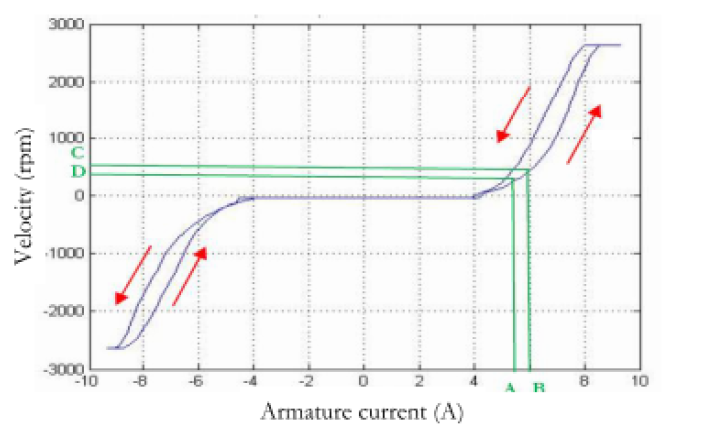
\includegraphics[width = .7\textwidth]{pics/RM_RPM_Current.png}
\caption{Rotational Velocity of the Right motor in function of the Current}
\label{fig:RM_RPM_curr}
\end{figure}

\begin{table}[H]
	\centering
		\begin{tabular}{c|c}
        \toprule
			Armature current [A] & Angular velocity [RPM] \\ \midrule
            5.4 & 244 \\
            5.7 & 370 \\
		\end{tabular}
	\caption{Operating points of the right motor}
	\label{tab:RM_operating_region}
\end{table}

\FloatBarrier

\section{Identifying the transfer function}
The transfer function was identified the same way the master motor was done: stepping from one operating point to another and measuring the step response. Using the least squares method a best fitting curve (figure \ref{fig:RM_id}) to the sampled data points was generated with a corresponding first order transfer function (equation \ref{eq:RM_TF}). 

\begin{align}
	G(s) = \frac{7.128}{6.0665S+1}
    \label{eq:RM_TF}
\end{align}

\begin{figure}[htbp]
\centering
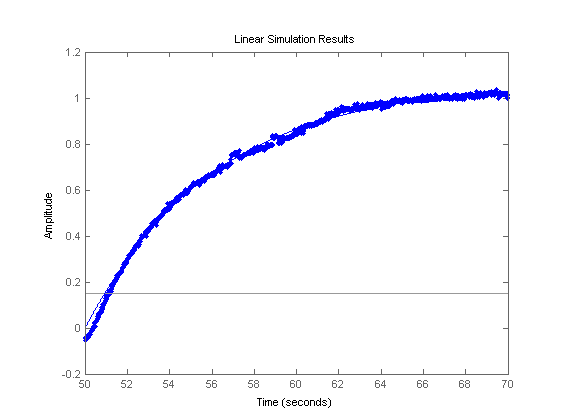
\includegraphics[width = 0.7\textwidth]{pics/RM_systemID.png}
\caption{Sampled data with the fitted curve from the calculated transfer function}
\label{fig:RM_id}
\end{figure}

\FloatBarrier
\section{Controller Design}
The controller for this motor needs to be fast enough to be able to keep the tension of the strip constant despite disturbances. To do this a proportional controller with gain $K$ was chosen. Figure \ref{fig:RM_rlocus} shows a root locus plot for the right motor. The gain can again be chosen arbitrarily.$K$ was chosen based on a couple simulations (figures \ref{fig:RM_K2_SIM}, \ref{fig:RM_K3_SIM} and \ref{fig:RM_K4_SIM}) and  practical experiments for different gains (figures \ref{fig:RM_K2}, \ref{fig:RM_K3} and \ref{fig:RM_K4}). None of the simulations have overshoot while some of the practical experiments do (depending on $K$). This is because the transfer function of the motor was reduced to a first order system while in practice it probably as a non linear system.

\begin{figure}[htbp]
\centering
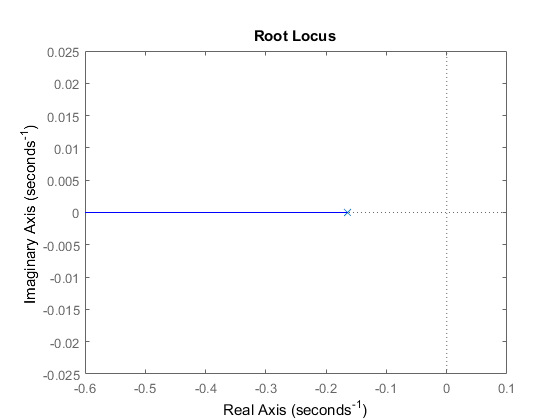
\includegraphics[width = \textwidth]{pics/RM_rlocus.png}
\caption{Root locus plot for the right motor}
\label{fig:RM_rlocus}
\end{figure}



A gain of $K = 3$ was used since using a higher gain has the risk of putting current output of the controller over the maximum current of the driver. In this case this would not be a problem since the maximum output of the DAC is 10 which is also the maximal input value of the motor driver. And since no integrator is used, no wind-up could occur. Using more extensive experiments a more aggressive setting of the controller (higher gain) could be achieved, but could possibly cause instability or oscillations around the set point.

\begin{figure}[htbp]
\centering
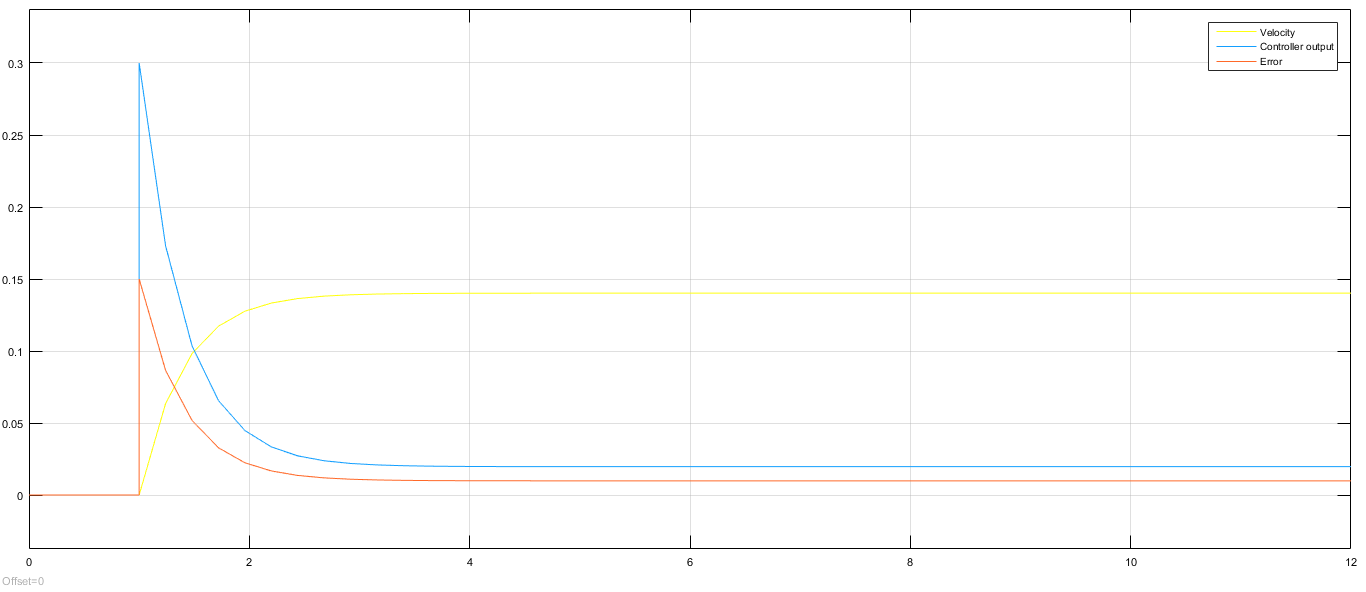
\includegraphics[width = \textwidth]{pics/RM_K2_SIM.png}
\caption{Simulink simulation of the right motor behaviour for $K = 2$}
\label{fig:RM_K2_SIM}
\end{figure}

\begin{figure}[htbp]
\centering
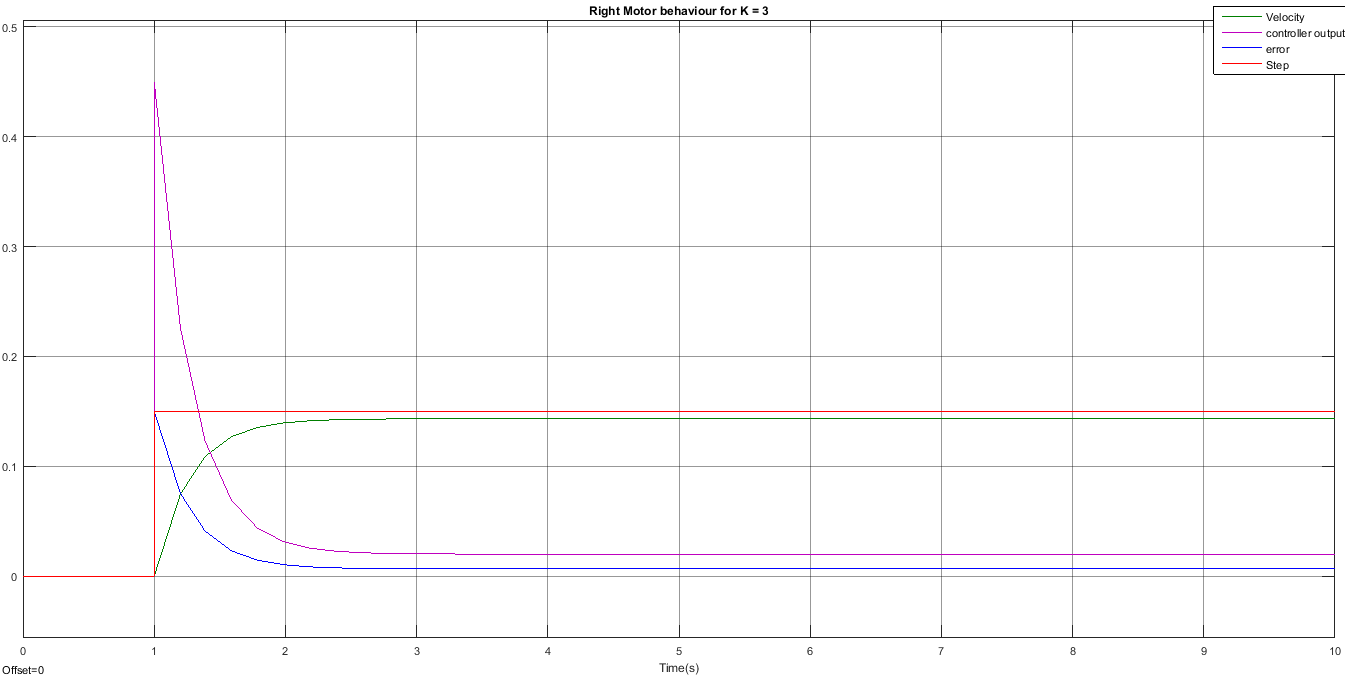
\includegraphics[width = \textwidth]{pics/RM_K3_SIM.png}
\caption{Simulink simulation of the right motor behaviour for $K = 3$}
\label{fig:RM_K3_SIM}
\end{figure}

\begin{figure}[htbp]
\centering
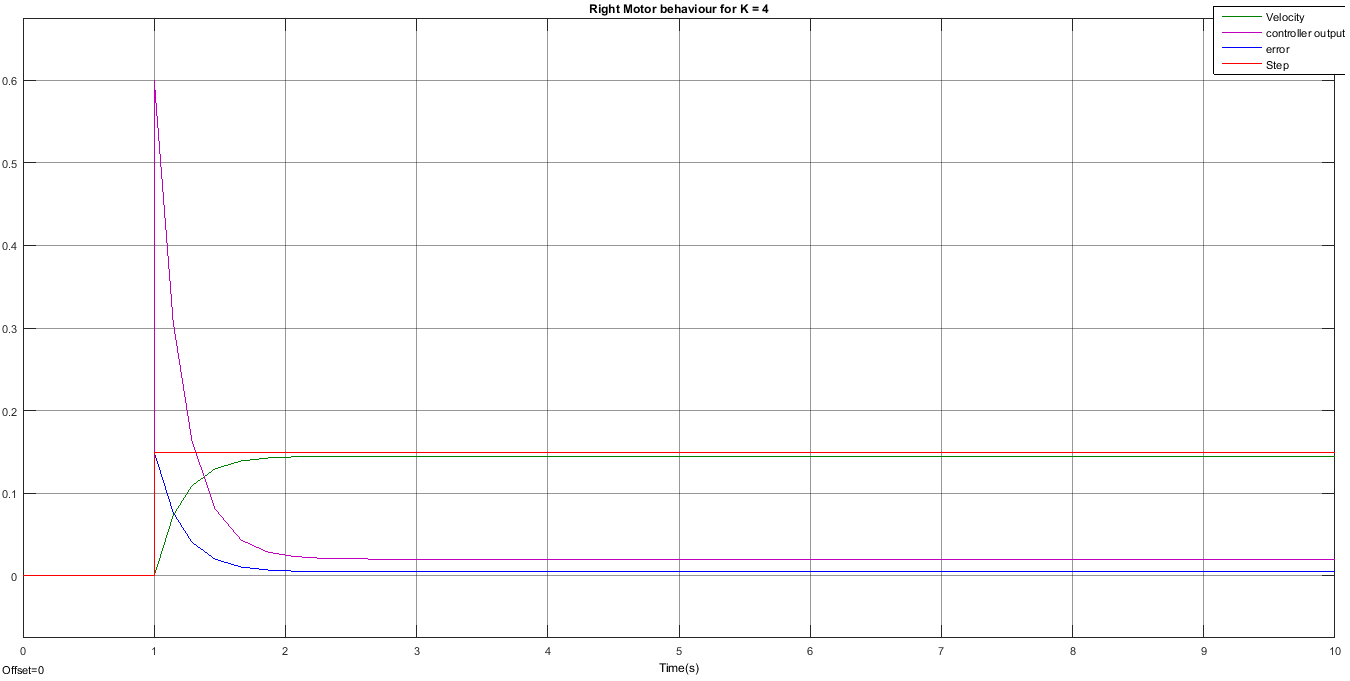
\includegraphics[width = \textwidth]{pics/RM_K4_SIM.png}
\caption{Simulink simulation of the right motor behaviour for $K = 4$}
\label{fig:RM_K4_SIM}
\end{figure}



\begin{figure}[htbp]
\centering
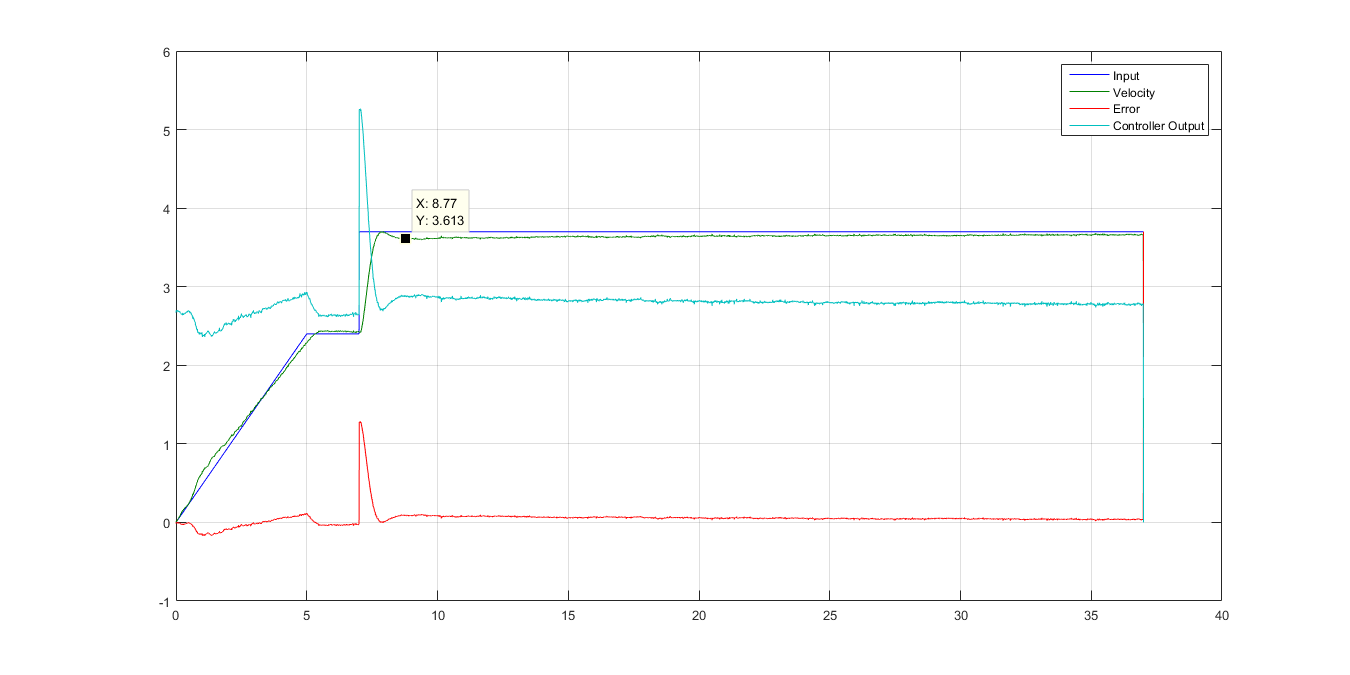
\includegraphics[width = \textwidth]{pics/RM_K2.png}
\caption{Response of the left motor behaviour for $K = 2$ to the blue curve as input.}
\label{fig:RM_K2}
\end{figure}

\begin{figure}[htbp]
\centering
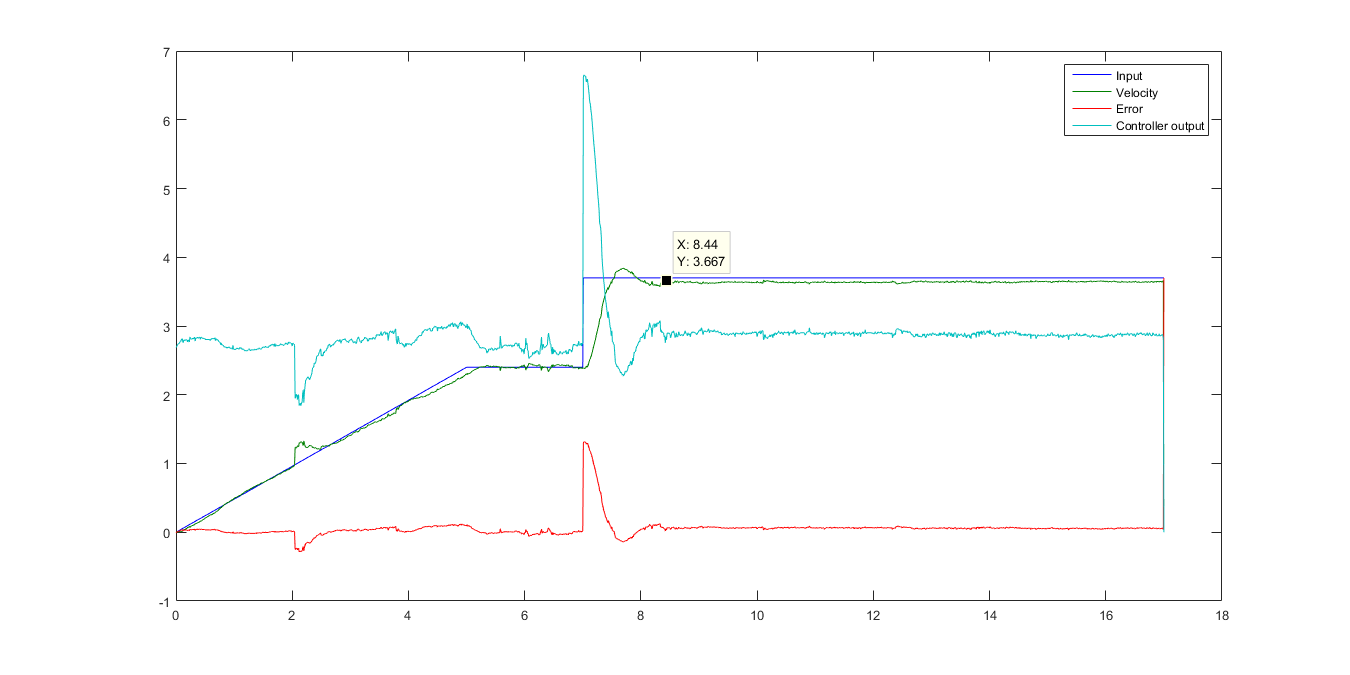
\includegraphics[width = \textwidth]{pics/RM_K3.png}
\caption{Response of the left motor behaviour for $K = 3$ to the blue curve as input.}
\label{fig:RM_K3}
\end{figure}

\begin{figure}[htbp]
\centering
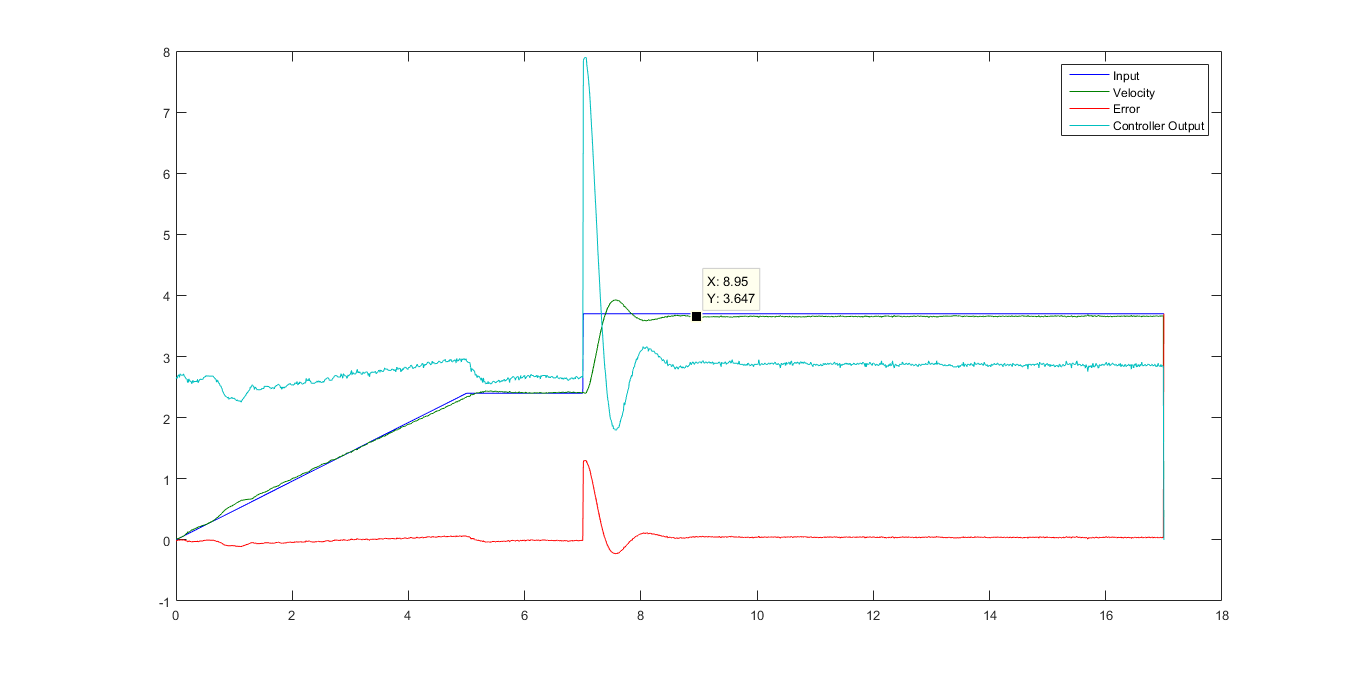
\includegraphics[width = \textwidth]{pics/RM_K4.png}
\caption{Response of the left motor behaviour for $K = 4$ to the blue curve as input.}
\label{fig:RM_K4}
\end{figure}


